%MARCOS RIAL DOCAMPO
%Parte del documento principal TFG

%%%%%%%%%%%%%%%
%% DISCUSIÓN %%
%%%%%%%%%%%%%%%

\chapter{Discusión}

Podemos concluir que para la obtención de firmas para realizar bibliotecas espectrales tomar solamente una observación de cada especie se trate de una metodología correcta. Pero a la hora de realizar un análisis de separabilidad espectral fiable y, sobre todo, para hacer el posterior volcado de los resultados del análisis a la clasificación de imágenes satélite, resultaba óptimo tener numerosas observaciones de una misma especie. De este modo se permitiría conocer más a fondo aspectos de cada especie como desviación estándar de las observaciones con un valor central para cada banda, que serían datos esenciales al hacer una clasificación supervisada de las imágenes Landsat.%\Sep

En cualquier caso, se preveía una dificultad el poder clasificar tres especies de mangle, que ya de por sí no están claramente separadas en el terreno, en una imagen de resolución espacial de 30 metros. Una posible solución a este problema sería el de tomar otro tipo de imagen satelital con mayor resolución espacial, como puede ser Spot o IKONOS, o realizar una fusión de imágenes combinando la mayor resolución espacial mencionada con la amplia resolución espectral de Landsat 8.%\Sep

Otro aspecto a tener en cuenta es el del software. Durante las distintas fases de realización del trabajo resultaron llamativas las numerosas actualizaciones que recibió el software. Y, aunque la mayoría fueron actualizaciones menores que no afectaban a funciones importantes del programa, cabe destacar que el cambio de versión no resultó un problema de compatibilidad de archivos provenientes de versiones anteriores. En el caso de GRASS durante la realización del \ac{TFG} se liberó la versión estable 7.0 solo presentando problemas de traducción haciendo confuso el uso de algún comando o proceso, pero en ningún caso presentó problemas de compatibilidad entre versiones, salvo los evidentes a la hora de abrir un proyecto hecho en la versión anterior.%\Sep

Para la realización de la clasificación de las imágenes Landsat 8 se estudió la utilización de un plugin de QGIS llamado \ac{SCP} que permite hacer una clasificación supervisada y aplicar índices de vegetación de forma guiada por una interfaz de usuario perfectamente integrada en el software. Este plugin, creado por \cite{Congedo2015}, permite aplicar los clasificadores \ac{SAM}, el \ac{MLC} y \ac{NN} además de ofrecer una alternativa para obtener imágenes Landsat a las ya mencionadas en capítulos anteriores. Con el \ac{SCP} podemos importar archivos de firmas espectrales de forma sencilla.%\Sep

Una posible forma de mejorar la clasificación sería la de crear una máscara para la zona de más interés centrando esta en la costa del Golfo adentrándose unos kilómetros al interior. Un modo de realizar y aplicar esta máscara sería gracias al comando \textit{r.mask} de GRASS donde la podremos crear a partir de una capa ráster o vectorial que tengamos digitalizada en el proyecto y aplicarla dentro de las opciones del comando de clasificación. Otro aspecto a tener en cuenta para mejorar el resultado es la de ser más exhaustivos en la creación de las áreas de entrenamiento. En este caso se consideró suficiente el aproximarse a una media de 4000 píxeles por clase para obtener un resultado aceptable y verosímil, pero un incremento del número de píxeles en algunas clases ayudaría a definir mejor la clasificación e incluso, de tener un mayor conocimiento de la zona, crear algunas nuevas clases. También se podría haber hecho un análisis de \ac{CP} de la imagen.%\Sep

Cabe destacar también en cuanto a GRASS la utilidad de la herramienta \textit{Map Swipe} (\textit{g.gui.mapswipe}) que permite una mejor comparación de dos mapas superpuestos creando una ``cortinilla'' como se muestra en la figura \ref{fig:map_swipe}. Esta herramienta se implementó en la versión 7.0.

\begin{figure}
	\centering
	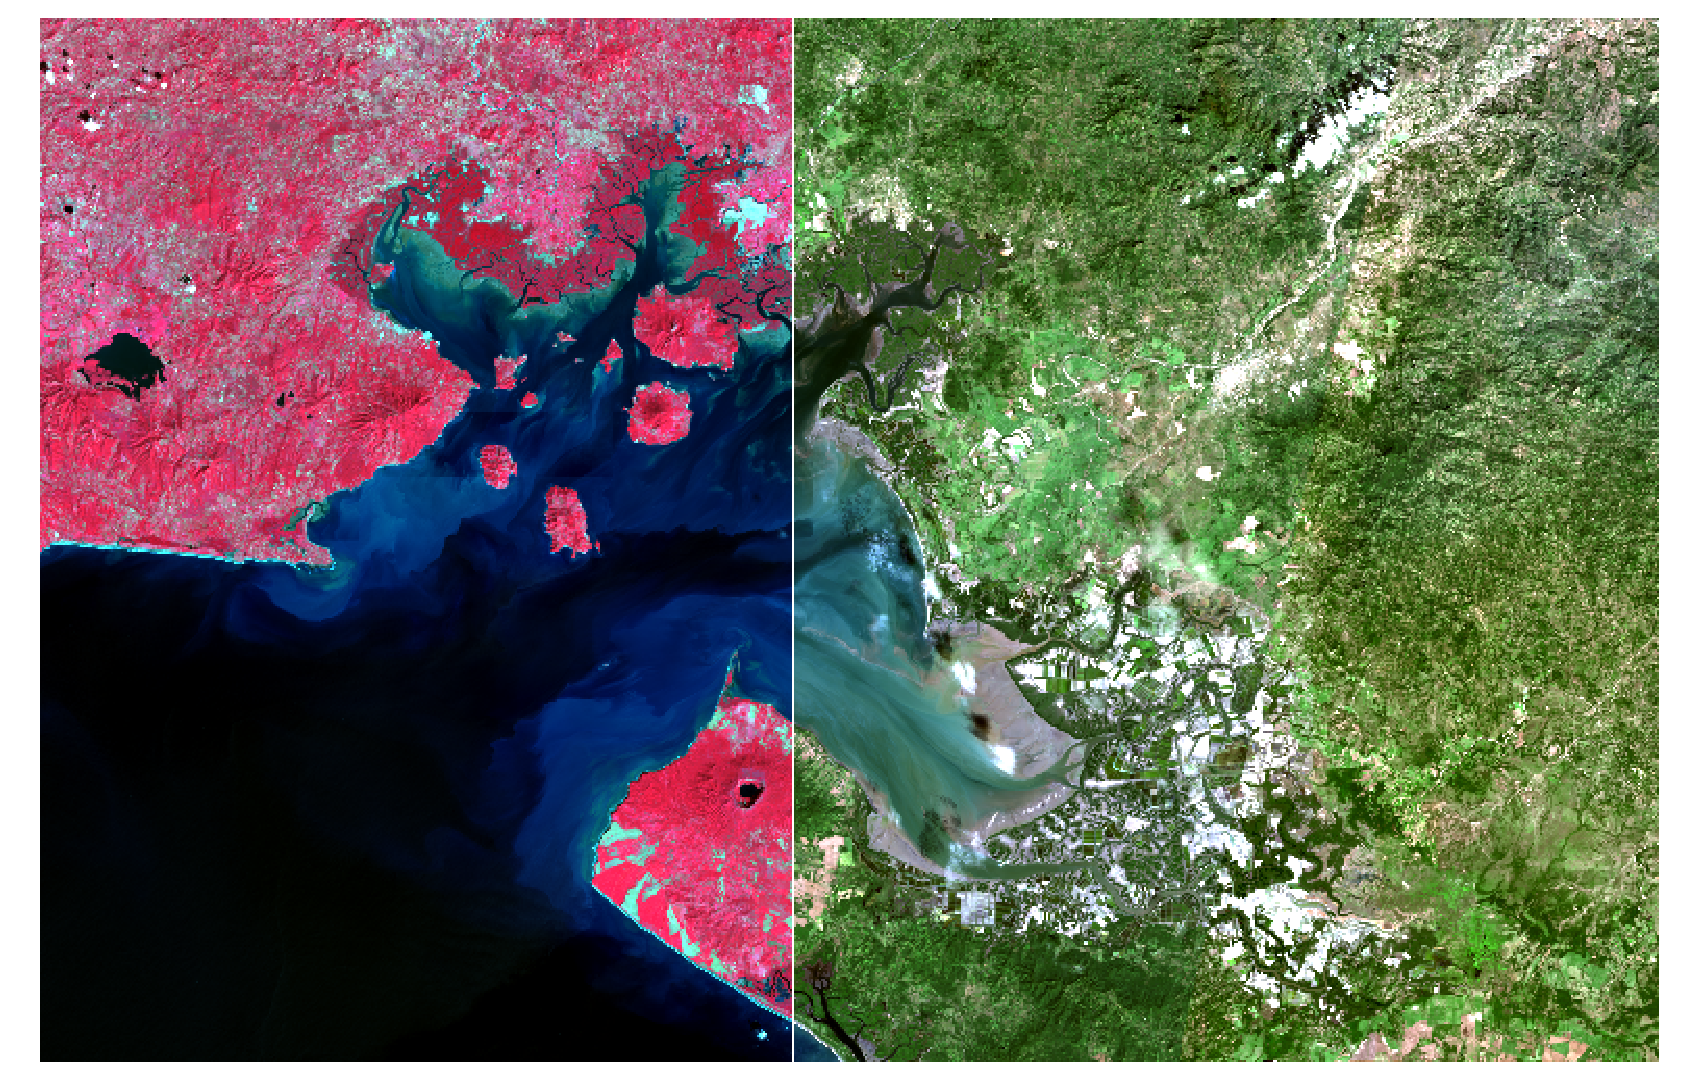
\includegraphics[width=0.9\linewidth]{./Imagenes/Map_swipe.eps}
	\captionsetup{font={footnotesize,it}}
	\caption[\textit{Map Swipe} de GRASS 7]{Ejemplo de \textit{Map Swipe} de GRASS 7. Se comparan combinaciones en falso color 5-4-3 y color real 4-3-2. Elaboración propia.}
	\label{fig:map_swipe}
\end{figure}